\subsection{SVM Results} A total of 16 different configurations of the SVM algorithm were studied, combining the four kernels mentioned in Section \ref{methodology-svm-sec} (linear, RBF, polynomial, and sigmoid) with four different values for the parameter $C$. After training and testing each configuration on the datasets, an initial preselection of the best models based on accuracy was conducted. A Friedman test was then performed to determine whether there were statistically significant differences in accuracy between the models. For each dataset (hepatitis and mushroom), the model with the highest accuracy was selected.

\subsubsection{Hepatitis} For this dataset, the five models with the highest mean accuracies were selected from the initial 16. The mean accuracies and hyperparameters of these models are presented in Figure \ref{fig:hep-svm-1}. A more in-depth analysis of these five models can be found in Table \ref{tab:svm_metrics}.

\begin{figure}[Ht]
    \centering
    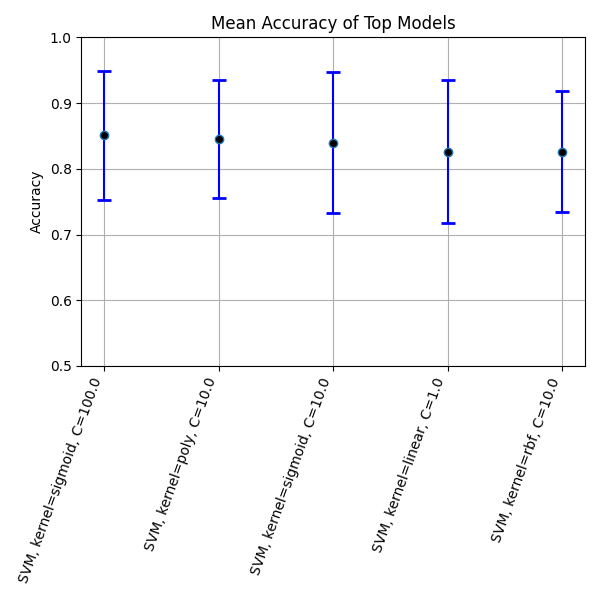
\includegraphics[width=0.5\textwidth]{figures/svm/hepatitis/statistical_analysis_results.png}
    \caption{Mean accuracy for the five models of SVM with higher mean accuracies.}
    \label{fig:hep-svm-1}
\end{figure}


\begin{table}[h!]
\centering
\begin{tabular}{|l|c|c|c|}
\hline
\textbf{Model} & \textbf{Accuracy} & \textbf{F1 Score} & \textbf{Time (s)} \\
\hline
SVM, kernel=sigmoid, C=100.0 & 0.851 $\pm$ 0.010 & 0.91 $\pm$ 0.06 & 0.0006 $\pm$ 0.0005 \\
\hline
SVM, kernel=poly, C=10.0     & 0.84 $\pm$ 0.09 & 0.91 $\pm$ 0.05 & 0.0008 $\pm$ 0.0005 \\
\hline
SVM, kernel=sigmoid, C=10.0  & 0.84 $\pm$ 0.11 & 0.90 $\pm$ 0.07 & 0.0005 $\pm$ 0.0007 \\
\hline
SVM, kernel=linear, C=1.0    & 0.82 $\pm$ 0.11 & 0.89 $\pm$ 0.07 & 0.0011 $\pm$ 0.0006 \\
\hline
SVM, kernel=rbf, C=10.0      & 0.82 $\pm$ 0.09 & 0.89 $\pm$ 0.06 & 0.0011 $\pm$ 0.0006 \\
\hline
\end{tabular}
\caption{Performance metrics for the best five SVM models with different kernels and regularization parameters.}
\label{tab:svm_metrics}
\end{table}

The Friedman test was performed, yielding a $p$-value of 0.4292, leading us to accept the null hypothesis that there are no significant differences between the five models studied. The model with hyperparameters kernel=sigmoid and C=100.0, as shown in Table \ref{tab:svm_metrics}, exhibited higher mean accuracy, a higher mean F1 score, and lower mean computation time. Therefore, this model will be considered for further analysis on the reduced datasets.

\subsubsection{Mushroom}

For this dataset, the ten models with the highest mean accuracies were selected from an initial set of sixteen. Although a larger number of models was considered in the preliminary analysis, no significant differences in accuracy were observed, with over five models achieving 100$\%$ accuracy. Consequently, the Friedman test could not be applied, as there was insufficient variance in the accuracies of the ten selected models. This lack of variability in performance metrics rendered the Friedman test ineffective for distinguishing among these top models. The values obtained for the studied metrics are shown in Table \ref{tab:svm_metrics_m}

\begin{table}[h!]
\centering
\begin{tabular}{|l|c|c|c|}
\hline
\textbf{Model} & \textbf{Accuracy} & \textbf{F1 Score} & \textbf{Time (s)} \\
\hline
SVM, kernel=linear, C=1.0    & 1.0000 $\pm$ 0.0000 & 1.0000 $\pm$ 0.0000 & 0.0031 $\pm$ 0.0005 \\
\hline
SVM, kernel=linear, C=10.0   & 1.0000 $\pm$ 0.0000 & 1.0000 $\pm$ 0.0000 & 0.0038 $\pm$ 0.0011 \\
\hline
SVM, kernel=rbf, C=100.0     & 1.0000 $\pm$ 0.0000 & 1.0000 $\pm$ 0.0000 & 0.0077 $\pm$ 0.0013 \\
\hline
SVM, kernel=linear, C=100.0  & 1.0000 $\pm$ 0.0000 & 1.0000 $\pm$ 0.0000 & 0.0034 $\pm$ 0.0006 \\
\hline
SVM, kernel=poly, C=10.0     & 1.0000 $\pm$ 0.0000 & 1.0000 $\pm$ 0.0000 & 0.0023 $\pm$ 0.0007 \\
\hline
SVM, kernel=poly, C=100.0    & 1.0000 $\pm$ 0.0000 & 1.0000 $\pm$ 0.0000 & 0.0021 $\pm$ 0.0005 \\
\hline
SVM, kernel=rbf, C=10.0      & 1.0000 $\pm$ 0.0000 & 1.0000 $\pm$ 0.0000 & 0.0087 $\pm$ 0.0022 \\
\hline
SVM, kernel=rbf, C=1.0       & 0.9994 $\pm$ 0.0010 & 0.9994 $\pm$ 0.0011 & 0.0245 $\pm$ 0.0025 \\
\hline
SVM, kernel=poly, C=1.0      & 0.9978 $\pm$ 0.0015 & 0.9977 $\pm$ 0.0016 & 0.0070 $\pm$ 0.0018 \\
\hline
SVM, kernel=linear, C=0.1    & 0.992 $\pm$ 0.004 & 0.992 $\pm$ 0.004 & 0.0060 $\pm$ 0.0017 \\
\hline
\end{tabular}
\caption{Performance metrics for various SVM models with different kernels and regularization parameters (C).}
\label{tab:svm_metrics_m}
\end{table}

